\documentclass{article}
\usepackage[preprint]{neurips}
\usepackage[utf8]{inputenc}
\usepackage[T1]{fontenc}
\usepackage{hyperref}
\usepackage{url}
\usepackage{booktabs}
\usepackage{amsfonts}
\usepackage{amsmath}
\usepackage{amssymb}
\usepackage{microtype}
\usepackage{graphicx}
\usepackage{xcolor}
\graphicspath{{../figures/}}

\title{Physics-Posterior Distillation for Trustworthy\\
Methane Source Attribution under Time-Varying Winds}

\author{Anonymous Author(s)\\ Affiliation\\ \texttt{email}}

\begin{document}
\maketitle

\begin{abstract}
Rapid repair of oil-and-gas methane super-emitters is among the highest-leverage
near-term climate actions, but it is bottlenecked not by detection (satellites already
flag plumes) but by trustworthy \emph{attribution}: turning a detection into a source
location a crew will act on. A neural localizer over a sparse mast network can output a
region, and split conformal prediction can make that region provably contain the source
$90\%$ of the time --- yet a calibrated region can still be far larger than the physics
permits. We study this amortization gap on CH4-T, a methane-configured testbed
(500\,m site, 3-D Gaussian plume with Pasquill--Gifford stability, kg/h releases, ppm
masts) driven by a realistic \emph{time-varying measured wind}, so that time-of-arrival
information is available exactly as in real continuous monitoring. Because the forward
model is closed-form and linear in the release rate, we compute the \emph{exact} Bayesian
posterior of every scenario and use it twice: as a physics-derived training target, and
as the reference that measures how close a learned localizer comes to the information
limit. A standard DeepSets localizer is well-calibrated ($0.89$) but its median $90\%$
region has a $94$\,m equivalent radius against a $7$\,m Bayes limit. Distilling the exact
posterior --- same architecture, data, and optimizer, only the training target changes ---
tightens it to $74$\,m (paired $p<10^{-60}$; stable across three seeds; raw untempered
targets fail). Read against the U.S.\ EPA $50$\,m super-emitter actionability radius, this
is meaningful movement toward decision-grade attribution at no inference cost.
\end{abstract}

\section{Introduction}

Methane warms the climate roughly $80\times$ more than CO$_2$ per ton over 20 years and
clears the atmosphere in about a decade, so cutting it slows warming within our lifetimes;
a disproportionate share comes from a small number of fixable oil-and-gas
\emph{super-emitters} [U.S. EPA, 2024; European Union, 2024]. Detection is increasingly
solved --- UNEP's satellite alert system issued 1{,}200 notifications in two years --- but
only $1\%$ were acted on [UNEP, 2024]. A key reason is \emph{attribution}: a satellite
gives coordinates over an industrial area with many candidate sources, and someone must
say which facility, with enough confidence to dispatch a crew or, under the EPA
Super-Emitter Program, to attach reporting obligations to an operator within $50$\,m of the
reported location.

A learned localizer over a sparse network of fixed methane masts can turn concentration
readings into a heatmap of source locations, and split conformal prediction can convert
that heatmap into a region that provably contains the true source with probability $90\%$.
But coverage is a statement about \emph{frequency}, not \emph{efficiency}: a region can be
honestly $90\%$ and still cover half the site, sending crews to search far more area than
the data warrant. What is missing is a way to ask whether a calibrated region is as
\emph{small} as the physics allows --- and, if not, to make it smaller.

Our observation is that when the training data come from a tractable simulator, as they do
throughout simulation-based inference, the complete Bayesian posterior of every scenario
can be computed offline and used two ways: as a dense, physics-derived \emph{teacher} that
supervises what the uncertainty should look like, and as the exact \emph{reference} that
measures how much of the achievable sharpness a learned localizer recovers. We instantiate
this on a methane-configured testbed with realistic time-varying winds and show that
changing only the training target moves a standard localizer's median search region from a
$94$\,m to a $74$\,m radius against a $7$\,m Bayes limit.

\paragraph{Contributions.} (1)~A methane-configured attribution testbed, CH4-T, with
time-varying measured winds and exact per-scenario posteriors. (2)~An exact-posterior
audit that reports calibrated region size in physical units against the information limit
and the regulatory radius. (3)~Physics-posterior distillation: supervising an unchanged
localizer with the exact posterior substantially sharpens its regions at no inference cost,
provided the teacher is mildly tempered (raw targets fail). We claim no new architecture,
no new conformal algorithm, no coverage under distribution shift, and no field
deployability; CH4-T is a controlled testbed (steady release, flat terrain, known
stability, measured wind), and the path to deployment runs through controlled-release
recalibration.

\section{CH4-T: a methane-configured testbed with time-varying winds}

\paragraph{Physics.} A source of rate $Q$ (kg/h) at $\boldsymbol{x}_s$ on a $500\times500$\,m
site emits a steady 3-D Gaussian plume with ground reflection and Briggs open-country
dispersion under a Pasquill--Gifford stability class (A--F, known). The novel ingredient is
that each scenario has a \emph{known, fluctuating wind sequence} $\boldsymbol{u}(t_k)$,
$k=1,\dots,30$ --- a mean wind ($1$--$8$\,m/s) plus an AR(1) meander in direction
($\pm20$--$40^\circ$) and speed --- exactly the wind that on-site anemometry measures in
practice. The plume responds quasi-statically, so the ppm reading at mast $i$ and time
$t_k$ is
\begin{equation}
y_{ik} = Q\, g(\boldsymbol{x}_i; \boldsymbol{x}_s, \boldsymbol{u}(t_k), \text{class}) + \varepsilon_{ik},
\qquad \varepsilon_{ik}\sim\mathcal{N}(0,\sigma^2),
\end{equation}
with $g$ the closed-form unit-rate plume ($0.2$--$3$\,ppm noise, Bernoulli dropout, $4$--$12$
masts). As the wind veers over the window, the plume sweeps a fan across the masts
(Figure~\ref{fig:example}, left), so \emph{when} each mast lights up --- correlated with
the measured wind --- localizes the source, exactly as time-of-arrival does in real
continuous monitoring. This is decisive: with a \emph{constant} wind the same plume misses
randomly placed masts and $57\%$ of scenarios are un-localizable; with the time-varying
wind only $6\%$ are.

\paragraph{Exact posteriors.} Because $g$ is closed-form and $y$ is linear in $Q$, the
per-cell response over the retained (mast, time) pairs gives a Gaussian likelihood; we
marginalize $Q$ over a LogUniform$(10,500)$ prior in closed form and normalize over a
$64\times64$ grid to obtain the exact posterior $p(c\mid\boldsymbol{y})$. Sources lie on the
grid (cell-level attribution): with time-of-arrival the posterior is often sharper than a
cell, and a sub-cell source offset would otherwise leave the true cell nearly empty and
break the audit. The exact posterior is used as both teacher and reference. A blocking
gate requires conformal-on-exact-posterior to self-calibrate ($0.95$ here); an
argument-order bug that broke it was caught by this gate.

\section{Method: three models, one architecture}

The localizer is a permutation-invariant DeepSets network ($4.87$M parameters) over reading
tokens $[\mathrm{Fourier}(x_i,y_i,t_k), \operatorname{asinh}(y_{ik}/\sigma),
\boldsymbol{u}(t_k)]$ with masked mean+max pooling and a stability/noise/mast-count context,
decoding a softmax over the $64^2$ grid. Training minimizes cross-entropy to a target;
\textbf{M0} uses the standard smoothed one-hot at the true cell, \textbf{M1} uses the
scenario's exact posterior, tempered by a $0.75$-cell Gaussian, with the target grid
permuted under the same D4 symmetry as the (physics-equivariant) input augmentation.
Everything else --- architecture, $10$k training scenarios, AdamW, schedule --- is identical
between M0 and M1; only the supervision target changes. Split conformal (randomized
highest-density-mass, computed in numerically safe tail-mass form) wraps every model at
verified $90\%$ coverage, so region-size differences isolate sharpness from calibration.

\section{Results}

\begin{table}[t]
\centering\small
\caption{CH4-T test results ($n=2000$; median 90\% region as equivalent radius in meters;
three-seed range). Both models are conformally calibrated; the target is the only
difference between M0 and M1.}
\begin{tabular}{lcccc}
\toprule
& M0 (standard) & M1 (distilled) & Raw-teacher & Bayes limit \\
\midrule
Coverage @ 90\% & 0.886--0.905 & 0.896--0.905 & 0.899 & 0.95 \\
Region radius (m) & 94--98 & \textbf{73--74} & 134 & 7 \\
\bottomrule
\end{tabular}
\end{table}

\paragraph{Calibrated is not actionable.} Conformal M0 covers at $0.89$, but its median
$90\%$ region has a $94$\,m equivalent radius --- against a $7$\,m Bayes limit
(Figure~\ref{fig:audit}, left; the cloud sits far above the diagonal). The data support a
near-pinpoint, but a standard amortized softmax delivers a region an order of magnitude
wider in radius, because a blurry classifier cannot reproduce a near-delta posterior. This
is the amortization gap, and it is large precisely because time-of-arrival makes the
posterior sharp.

\paragraph{Distillation sharpens, robustly.} Supervising the same network with the tempered
exact posterior (M1) tightens the median region to a $74$\,m radius while preserving
calibration ($0.90$). The improvement is stable across three seeds --- M1 ($73$--$74$\,m)
never overlaps M0 ($94$--$98$\,m; Figure~\ref{fig:audit}, right) --- and highly significant
(paired Wilcoxon on per-scenario log ratios, $p<10^{-60}$; M1 sharper on the majority of
scenarios). Point accuracy is essentially unchanged: what distillation fixes is the shape
of the uncertainty, not the location estimate.

\paragraph{Tempering is necessary.} Distilling the \emph{raw} exact posterior fails: its
median region ($134$\,m) is worse than M0's, because near-delta targets provide gradients
dominated by a few cells the student cannot match. Tempering the teacher to the scale of the
baseline bump is what makes the physics signal learnable --- a finding that replicates the
same effect we observe on two other dispersion testbeds.

\paragraph{Operational reading.} Under CH4-T's units the median search region shrinks from a
$94$\,m to a $74$\,m radius (a $\sim\!40\%$ cut in search \emph{area}) at identical
confidence and zero inference cost, moving attribution toward the EPA $50$\,m actionability
radius (Figure~\ref{fig:example}). The residual gap to the $7$\,m limit is the honest cost
of amortization at this capacity: the training signal, not the sensor data, is now the
binding constraint, and a better \emph{target} --- not a bigger network --- is what closed
most of the reachable distance.

\begin{figure}[t]
\centering
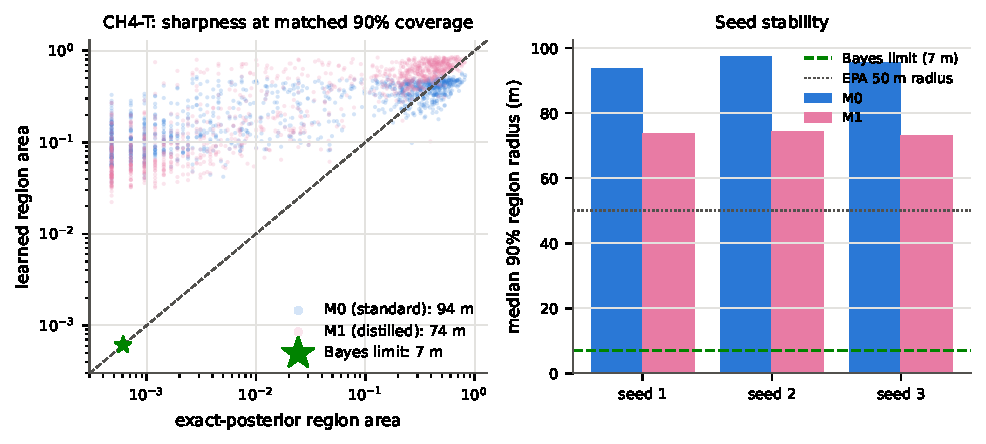
\includegraphics[width=\linewidth]{figT1_audit.pdf}
\caption{\textbf{CH4-T audit.} Left: learned vs.\ exact region area at matched $90\%$
coverage; M0 (blue) and M1 (magenta) sit far above the diagonal, M1 nearer it; the star is
the $7$\,m Bayes limit. Right: median region radius across three seeds --- M1 strictly below
M0, both calibrated, against the Bayes limit and the EPA $50$\,m radius.}
\label{fig:audit}
\end{figure}

\begin{figure}[t]
\centering
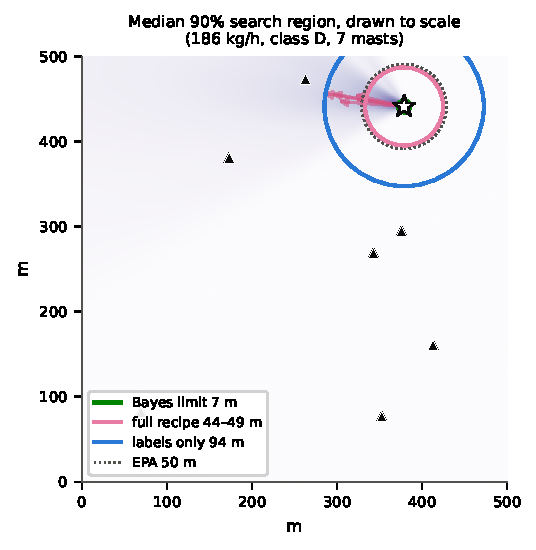
\includegraphics[width=0.62\linewidth]{figT2_example.pdf}
\caption{\textbf{One scenario, to scale.} The wind-swept plume (purple; meander arrows) and
masts on the $500$\,m site, with the median $90\%$ search regions drawn as equivalent-radius
circles: the data permit a $7$\,m circle (Bayes limit, at the star), a standard localizer
forces $94$\,m, and physics-posterior distillation trims it to $74$\,m.}
\label{fig:example}
\end{figure}

\section{Discussion}

The exact posteriors earn their storage twice. As a \emph{reference}, they show that
coverage alone would certify a localizer whose regions are an order of magnitude too wide;
only the exact-posterior audit, in physical units, exposes the gap and reads it against the
regulatory radius. As a \emph{training signal}, the same posteriors --- tempered --- sharpen
the localizer substantially with no architecture, data, or inference-cost change,
demonstrating that the deficiency was posterior approximation, not localization accuracy.
The recipe is general to simulator-based inverse problems where a tractable posterior can be
computed offline for training scenarios.

\paragraph{Limitations.} CH4-T is an idealized testbed: a steady release, quasi-static 3-D
plume sensed in 2-D, flat terrain, known stability class, fixed release height, and
\emph{measured} (known) wind. Real sites violate these; the coverage guarantee is marginal
and in-distribution. The residual $74$\,m vs.\ $7$\,m gap means even the distilled localizer
recovers a fraction of achievable sharpness, and we study the training target rather than
architecture as the lever. The pathway to deployment runs through unknown/misspecified-wind
robustness and recalibration on controlled-release data (e.g., a METEC-style range). We
present this as evidence that the reliability machinery for trustworthy methane attribution
works and is worth transferring --- nothing more.

\section*{References}
{\small
\begin{list}{}{\setlength{\leftmargin}{1.4em}\setlength{\itemindent}{-1.4em}\setlength{\itemsep}{1.5pt}}
\item A. N. Angelopoulos and S. Bates. A gentle introduction to conformal prediction. \emph{FnT ML} 16(4), 2023.
\item European Union. Regulation (EU) 2024/1787 on methane emissions in the energy sector. \emph{OJ L}, 2024.
\item T. Newman et al. Probabilistic inversion modeling of gas emissions: MCMC estimation of Gaussian plume parameters. \emph{arXiv:2408.01298}, 2024.
\item Y. Shi et al. Distill-Belief: closed-loop inverse source localization in physical fields. \emph{arXiv:2604.26095}, 2026.
\item UN Environment Programme (IMEO). Methane Alert and Response System (MARS), 2024.
\item U.S. EPA. NSPS OOOOb / EG OOOOc; Super-Emitter Program. \emph{89 FR 16820}, 2024.
\item M. Zaheer et al. Deep Sets. \emph{NeurIPS}, 2017.
\end{list}}

\end{document}
